\documentclass[12pt, a4paper]{article}
\usepackage[utf8]{inputenc}
\usepackage[french]{babel}
\usepackage{amsfonts}
\usepackage{graphicx}
\usepackage{fancyhdr}
\usepackage{url}
\usepackage[usenames,dvipsnames]{color}

\usepackage[top=3.3cm, bottom=3.3cm, left=2cm, right=2cm]{geometry}

\renewcommand{\baselinestretch}{1.2}

\pagestyle{fancy}
\usepackage{lastpage}
\renewcommand\headrulewidth{1pt}
\fancyhead[L]{Image UpScaling}
\fancyhead[R]{INSA de Rouen}
\renewcommand\footrulewidth{1pt}
\fancyfoot[C]{\textbf{Page \thepage/\pageref{LastPage}}}
\fancyfoot[R]{\includegraphics[width=0.10\textwidth]{Images/Logo_INSA.png}}

\title{Rapport de projet}
\author{Ophélie Guenoux \\Olivier Petit}
\date{Janvier 2016}

\begin{document}

\makeatletter
\begin{titlepage}
  \begin{center}
      \includegraphics[width=0.20\textwidth]{Images/Logo_INSA.png}
      \hfill
      \includegraphics[width=0.25\textwidth]{Images/logoasi.png}\\
    \vspace{1cm}
		\Huge \underline{\@title} 
			\\ \textsc{Image UpScaling}
			\\ \Large Projet d'Approfondissement et d'Ouverture
			\vspace{1cm}
			\begin{figure}[h!]
				\centering
				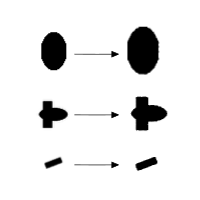
\includegraphics[width=0.5\textwidth]{Images/page-de-garde.png}
			\end{figure}
	\vspace{4cm}
	\end{center}
	\raggedright
	\large Ophélie Guenoux \hfill Encadrant : M.Chatelain \& M.Herault
	\\Olivier Petit \hfill INSA Rouen ASI4
	
\end{titlepage}

\newpage
\tableofcontents
\newpage

\vspace*{5cm}

\section*{Introduction}

Dans le cadre de notre projet PAO du semetre 7 en ASI (Architecture des systèmes d'informations), nous avons décidé de travailler sur la problématique d'agrandissement d'images matricielles à l'aide de réseaux de neurones artificiels.
\\

Ce projet a été l'occasion pour nous de découvrir de nouvelles techniques d'apprentissage automatique, avec en particulier l'utilisation des réseaux de neurones que nous n'avons pas encore étudiés.
\\

Dans ce rapport nous revenons sur les différentes étapes et la démarche que nous avons mis en place pour résoudre ce problème. Nous commencerons par expliquer brièvement ce qu'est l'image scaling, pour ensuite aborder le choix de la librairie utilisée. Finalement, nous parlerons des différentes parties de notre réalisation et expliciterons les problèmes que nous avons pu rencontrer.


\newpage

\section{L'image Scaling}

\subsection{Définition}
L'\textit{image scaling} est l'expression anglaise désignant les procédés informatiques liés à l'agrandissement ou la réduction de la taille d'une image.

Il existe deux familles d'images, les images vectorielles et les images matricielles.

Dans le cas d'images vectorielles l'agrandissement et la réduction sont effectués par le calcul de l'image à partir d'équations géométriques (points, courbes, droites, ...), stockées dans un fichier. De cette manière nous pouvons obtenir une image ``lisse'' quelque soit le coefficient d'échelle appliqué. Malheureusement peu d'images peuvent être représentées sous un ensemble de formes géométriques. C'est la raison pour laquelle les images vectorielles sont réservées à la création de diagrammes ou parfois de logos. Les images matricielles restent largement plus répandues.

Ce type d'image consiste en une matrice de trois dimensions, la largeur, la hauteur, et les trois ou quatre canaux de couleurs. Plus le nombre de pixels stockés est élevé, plus l'image est détaillée mais elle est également plus lourde. Des algorithmes de compressions permettent de faciliter le stockage et la transmission de celle-ci. Il s'agit par exemple, des formats comme JPEG, PNG, GIF, ...

Les images matricielles sont aujourd'hui bien plus répandues. Cependant, il peut être nécessaire dans certains cas de modifier la taille d'une image. Par exemple pour s'adapter aux différents types d'écrans ; avec en particulier l'augmentation de leur résolution. Certaines images doivent être agrandies pour être affichées correctement.

\begin{figure}[h!]
  \centering
  \includegraphics[scale=0.7]{Images/tele.png}
  \caption{Upscaling x2}
\end{figure}

\subsection{Agrandissement}
 
L'augmentation de la taille d'une image revient à "créer" de nouveaux pixels qu'il faudrait remplir le mieux possible afin de garder une continuité. Il faut donc ajouter de l'information que l'on ne connaît pas à la base. Il existe des algorithmes permettant de ``prédire'' la valeur des pixels a crées.

L'algorithme le plus simple est celui du plus proche voisin. Il est très rapide mais fourni un résultat pixélisé. C'est le plus répandu pour l'agrandissement ``à la volé''. Par exemple les visionneuses d'images l'utilisent.

\begin{figure}[h!]
  \centering
  \includegraphics[scale=0.6]{Images/plus_proche_voisin.png}
  \caption{Algorithme du plus proche voisin}
\end{figure}

De très nombreux algorithmes plus puissant existent, certain développés par de grandes entreprises. Une liste exhaustive est disponible ici:

\url{https://en.wikipedia.org/wiki/Image_scaling#Pixel_art_scaling_algorithms}

\subsection{Réduction}

La réduction d'une image est un procédé plus simple car il consiste généralement à supprimer des pixels de façon régulière(par exemple un sur deux). Il n'existe pas vraiment de problèmes liés à ces algorithmes car ils sont très simples à mettre en œuvre et l'exécution est peu complexe. Il forcement plus simple d'éliminer de l'information que d'en créer.


\section{Choix de la librairie}

Pour notre projet, nous souhaitions agrandir des images avec un réseau de neurones. Il s'agit effectivement d'un problème de machine learning pour son aspect prédictif. En effet le but est de prévoir la valeur des pixels à remplir. De ce fait, nous avons commencé à nous renseigner sur les différentes librairies de machine learning proposant des réseaux de neurones. \\ Parmi elles, Pylearn2 qui nous avait été justement conseillé par nos encadrants. 

\subsection{Theano et Pylearn2}
Notre choix s'est donc rapidement orienté vers Pylearn2 une librairie opensource sous license BSD qui utilise Theano (librairie machine learning reconnue). La librairie est en python, langage que nous connaissons. 
\\

Pylearn2 est avant tout une librairie de machine learning permettant de résoudre des problèmes de toutes sortes.(Clustering, classification, etc...).

Nous nous sommes intéressés à son implémentation de fonctions liées à la création de réseaux de neurones artificiels. Il s'agit de la classe MLP (\emph{multi layers perceptron}), qui contient toutes les types de couches connues. \\ Par exemple, dans le code suivant, nous créons un réseau de neurones contenant une couche de 75 neurones avec comme fonction d'activation une \emph{Sigmoid}

\begin{verbatim}
"model": !obj:pylearn2.models.mlp.MLP {
  "layers": [
   !obj:pylearn2.models.mlp.Sigmoid {
     layer_name: 'h1',
     dim: 75,
     irange: .5,
   },
 ]
}
\end{verbatim}

\subsection{Utilisation de \emph{YAML} avec Python}
Pylearn2 permet la définition d'un modèle de machine learning grâce à un script en \emph{YAML}.\\ L'exemple précédent est un extrait du script \emph{YAML} utilisé dans notre projet. 
\\

Initialement, pour bien comprendre le fonctionnement de la bibliothèque, nous avions réalisé une première version du projet uniquement avec des scripts Python. 
\\ Cependant, nous nous sommes très vite rendu compte des limites que cela engendraient. En effet, le code était devenu lourd et difficile à utiliser. 
\\

Par la suite, nous avons donc utilisé \emph{YAML} avec Python comme proposé par Pylearn2. Le côté architecture du réseau de neurones centralisé dans les scripts \emph{YAML} et le reste géré par les scripts Python. 

\section{Les différentes étapes du projet}
	\subsection{Le Dataset}
		\subsubsection{Construction}
Au commencement du projet, il était question de faire un Dataset composé de chiffres allant de 0 à 9. 
Cependant, nous avons vite été confronté à un problème: sa taille. En effet, celui-ci n'était composé que de 50 éléments, ce qui est largement insuffisant pour que l'apprentissage soit efficace.
\\

 Nous avons donc décidé de changer les données utilisées en images 32 pixels par 32, noir et blanc, représentant des ellipses et des rectangles.
\\Afin de contrer le problème de la taille du Dataset, nous avons crée un script Python capable de générer des images aléatoires en faisant varier la taille de l'objet, son inclinaison et sa position dans l'image générale. Grâce à cette méthode, nous avons réussi à avoir un Dataset de 2000 images. 
		\subsubsection{Utilisation}
Une fois ces images obtenues, nous avons besoin de créer un objet \emph{DenseDesignMatrix} qui pourra être ensuite utilisé par Pylearn2.\\ Cet objet sera  sérialiser sous la forme d'un fichier pickel puis désérialiser grâce à la ligne de code suivante :
\begin{verbatim}
"dataset": &train !pkl: "dataset_app.pkl",
\end{verbatim}
pour ensuite être utiliser lors de l’entraînement du réseau. 

 
	\subsection{Utilisation de Patchs}
	% mettre des images en entier sur le réseau -> beaucoup trop lent. Du coup réduction de la taille du réseau en ne passant que les patchs
	% deux nouveaux algo pour découper l'image en patch et pour la reformer
Les images que nous utilisons sont de taille 32 par 32 pixels. Au départ, nous avions pensé créer un réseau avec une entrée de dimension $32 \times 32 = 1024$ pour avoir en sortie une image agrandie $40 \times 40 = 1600$. Cependant, les résultats n'étaient pas concluant et la taille du réseau rendait l'apprentissage très long. Nous avons donc émis l'hypothèse que découper les images en patchs, avant de les mettre dans le réseau donnerait de meilleur résultats.
\\

Après avoir soumis l'idée à nos encadrants, nous avons pris la décision de découper les images d'entrées en patchs de taille $8 \times 8$ avec un recouvrement de moitié. Afin d'obtenir le même nombre de patchs en entrée et en sortie, nous avons pris des patchs de sortie de $10 \times 10$ produisant ainsi une image finale de taille $40 \times 40$.\\ Puis, on reconstruit l'image en superposant les patchs avec toujours un recouvrement de moitié et en faisant la moyenne des valeurs des pixels qui se recouvrent. 
\\

Finalement nous utilisons une fonction de seuillage pour éviter d'obtenir des valeurs inférieures à zéro ou supérieur à 255.

	\subsection{Structure du réseau}
	% nb couche
Au début du projet, nous avions fait un certain nombre de recherches sur le fonctionnement et la mise en place d'un réseau de neurones. Malheureusement, il est très difficile de trouver une architecture adéquate du premier coup sans avoir une certaine expérience. \\
Nous avons donc fait nos premiers choix par rapport à ce que nous avions lu durant nos recherches: choix du nombre de couches, du nombres de neurones et choix des fonctions d'activations. 

Cependant, lors de ces premiers essais, nous utilisions des fonctions d'activation génériques (\emph{Sigmoid} notamment), sans vraiment tenir compte de l'ensemble d'arrivée de celle-ci. 
Nous avons donc du retravailler à plusieurs reprises l'architecture de notre réseau, pour finalement arrivé à une architecture qui selon est assez satisfaisante. 

	\subsubsection{Les fonctions d'activation}
	% erreur de domaine de nos données, SIgmoid prend entre -inf et +inf pour ressortir en 0 et 1 ; 
	% ajouter un shéma pour expliquer les différentes couches
Initialement, nous avions décidé de construire un réseau de neurones avec deux couches et d'utiliser la même fonction d'activation pour chacune d'elles : une \emph{Sigmoid}.

Cependant l'ensemble de définition d'une \emph{Sigmoid} est de $-\infty$ à $+\infty$ et l'ensemble d'arrivé variant de 0 à 1. En sortie de la première couche les valeurs étaient donc comprise entre 0 et 1. Donc à la sortie de la seconde couche les données étaient entre 0.5 et 1 ce qui n'est pas satisfaisant. 

\begin{figure}[h!]
  \centering
  \includegraphics[scale=0.4]{Images/sigmoid.png}
  \caption{Fonction Sigmoid}
\end{figure}

Finalement au bout de plusieurs essais, notre réseau possède l'architecture suivante:
Tout d'abord une couche \emph{Sigmoid}, puis une \emph{RectifiedLinear} et enfin, une \emph{GaussianLinear} en couche de sortie.
\\

La première couche utilise des \emph{Sigmoid} donc les valeurs de sorties sont comprisent entre 0 et 1, comme expliqué précédemment.

La seconde couche utilise la fonction d'activation \emph{RectifiedLinear}. Cette fonction est simplement une rampe dans $[0 , +\infty[$ sinon 0. Elle peut donc être définite comme ceci:
$$f(x) = \left\{
        \begin{array}{ll}
          x & \mbox{si } x \in [0;+\infty[ \\
          0 & \mbox{sinon.}
        \end{array}
      \right.$$
 Les données en sorties sont donc encore entre 0 et 1.

 \begin{figure}[h!]
  \centering
  \includegraphics[scale=0.4]{Images/rectified.png}
  \caption{Fonction RectifiedLinear}
\end{figure}

La couche de sortie est un peu différente. Il s'agit d'une fonction linéaire comme la fonction présenté juste avant, mais qui ``passe'' à travers une loi normale. En réalité $$ y \sim p(y | x) = N(y | Wx+b, \beta^{-1}) $$ donc y suit une loi conditionnelle normale de moyenne $Wx+b$ et de variance $\beta^{-1}$.

$\beta$ est un paramètre supplémentaire qui doit être recalculé lors de l'algorithme de la descente du gradient.

	\subsubsection{Les différentes couches}
	
Durant la majorité du projet, nous étions sur un réseau en deux couches, comme évoqué précédemment. Avec une couche caché, dite \emph{hidden}, et la couche de sortie. 

Puis, suite à nos tests, nous avons conclue qu'un réseau en trois couches serait plus efficace. Le réseau actuel, est donc composé de trois couches: 

\begin{center}
\begin{tabular}{|l|c|r|}
  \hline
  couche & dimension & fonction d'activation\\
  \hline
  1 & 75 & Sigmoid \\
  2 & 90 & RectifiedLinear \\
  3 & 100 & LinearGaussian \\
  \hline
\end{tabular}
\end{center}

Voici finalement, un extrait du fichier YAML qui déclare les différentes couches :

\begin{figure}[h!]
\begin{verbatim}
"layers": [
      !obj:pylearn2.models.mlp.Sigmoid {
         layer_name: 'h1',
         dim: 75,
         irange: .5,
       },
       !obj:pylearn2.models.mlp.RectifiedLinear {
          layer_name: 'h2',
          dim: 90,
          irange: .5,
          max_col_norm: 1.0,
        },
        !obj:pylearn2.models.mlp.LinearGaussian {
           init_bias: !obj:pylearn2.models.mlp.mean_of_targets { dataset: *train },
           init_beta: !obj:pylearn2.models.mlp.beta_from_targets { dataset: *train },
           min_beta: 1.,
           max_beta: 100.,
           beta_lr_scale: 1.,
           dim: 100,
           layer_name: 'y',
           irange: .5,
       }
\end{verbatim}
  \caption{Architecture du réseau final}
\end{figure}


Le réseau est entraîné par l'algorithme de la descente du gradient (SGD : \emph{Stochastic Gradient Descent}). 

\begin{figure}[h!]
\begin{verbatim}
  "algorithm": !obj:pylearn2.training_algorithms.sgd.SGD {
      "learning_rate" : 0.001,
      "batch_size" : 1,
      "monitoring_batches" : 1,
      "monitoring_dataset": {
         "train": *train,
         "valid": !pkl: "dataset_val.pkl",
      },
      "termination_criterion": !obj:pylearn2.termination_criteria.EpochCounter {
         "max_epochs": 1000,
      },
      learning_rule: !obj:pylearn2.training_algorithms.learning_rule.AdaGrad {},
   }
\end{verbatim}
  \caption{Déclaration de l'algorithme d'apprentissage}
\end{figure}




\newpage
\section{Problèmes rencontrés}
Durant le déroulement du projet nous avons rencontrés quelques difficultés, en voici les principales. 
	\subsection{Le problème du pas}
Afin de mieux se rendre compte des résultats obtenus, nous avons utilisé \emph{LiveMonitor}, outil disponible dans Pylearn2 permettant de tracer les courbes d'apprentissage et de validation. 

Grâce à cet outil, nous avons tout d'abord remarqué que nos erreurs (apprentissage et validation) ne tombaient pas à 0 mais stagnaient plutôt autour d'une certaine valeur. Valeur qui pouvait changer en fonction du \emph{learning rate}. 
Nous avons donc utilisé deux approches pour tenter de corriger ce problème:

La première, travailler sur le \emph{learning-rate} de manière "brutale", en baissant tout simplement celui-ci une fois arrivé dans un certaine fourchette d'epochs. 

La seconde en utilisant un algorithme plus "intelligent", qui regarde un channel et une valeur de sortie et fait augmenter ou diminuer le \emph{learning rate} par rapport à cette valeur. Cette seconde approche s'est évéré la plus efficace. (voir code en dessous)
\\

Malgré plusieurs tentatives, nous n'avons pas réussi à corriger entièrement ce problème, nous l'avons juste diminuer fortement.

\begin{verbatim}
!obj:pylearn2.training_algorithms.sgd.MonitorBasedLRAdjuster {
    "high_trigger": 0.95,
    "low_trigger": 0.0,
    "grow_amt": 2,
    "shrink_amt": 0.5,
    "max_lr": 0.3,
    "min_lr": 0.000000001,
    "dataset_name": 'valid',
    "channel_name": 'valid_y_mse'
 },
\end{verbatim}
	
	\subsection{Upscalling-RGB}
Étant relativement satisfait des résultats obtenus, nous avons décidé d'adapter notre code pour pouvoir faire la même chose avec des images RGB. 

Nous avons donc repris la fonction \emph{upscalling}, pour la transformer en \emph{upscalling-RGB}. Concrètement, on applique notre traitement "upscalling" sur chacun des channels. 

Comme prévu, le résultat n'était pas celui attendu. En effet, il semble que les couleurs sont mal pris en compte, on obtient quelque chose de très bleu. 

\begin{center}
\begin{tabular}{cc}
   \includegraphics[scale=2]{Images/rectangleR_original.png} &
   \includegraphics[scale=2]
   {Images/rectangleR_reconstruction.png} \\
\end{tabular}
\end{center}

\begin{center}
\begin{tabular}{cc}
   \includegraphics[scale=0.5]{Images/oiseau_original.png} &
   \includegraphics[scale=0.5]
   {Images/oiseau_reconstruction.png} \\
\end{tabular}

\end{center}

\section*{Conclusion}
\end{document}
